\documentclass[../main.tex]{subfiles}
\graphicspath{{\subfix{../images/}}}
\begin{document}
\index{exercises!sitting meditation}
\label{Ex:SittingMed}
\noindent
\begin{tabular}{p{1.8cm} p{9.7cm} }
 \raisebox{-1\totalheight}{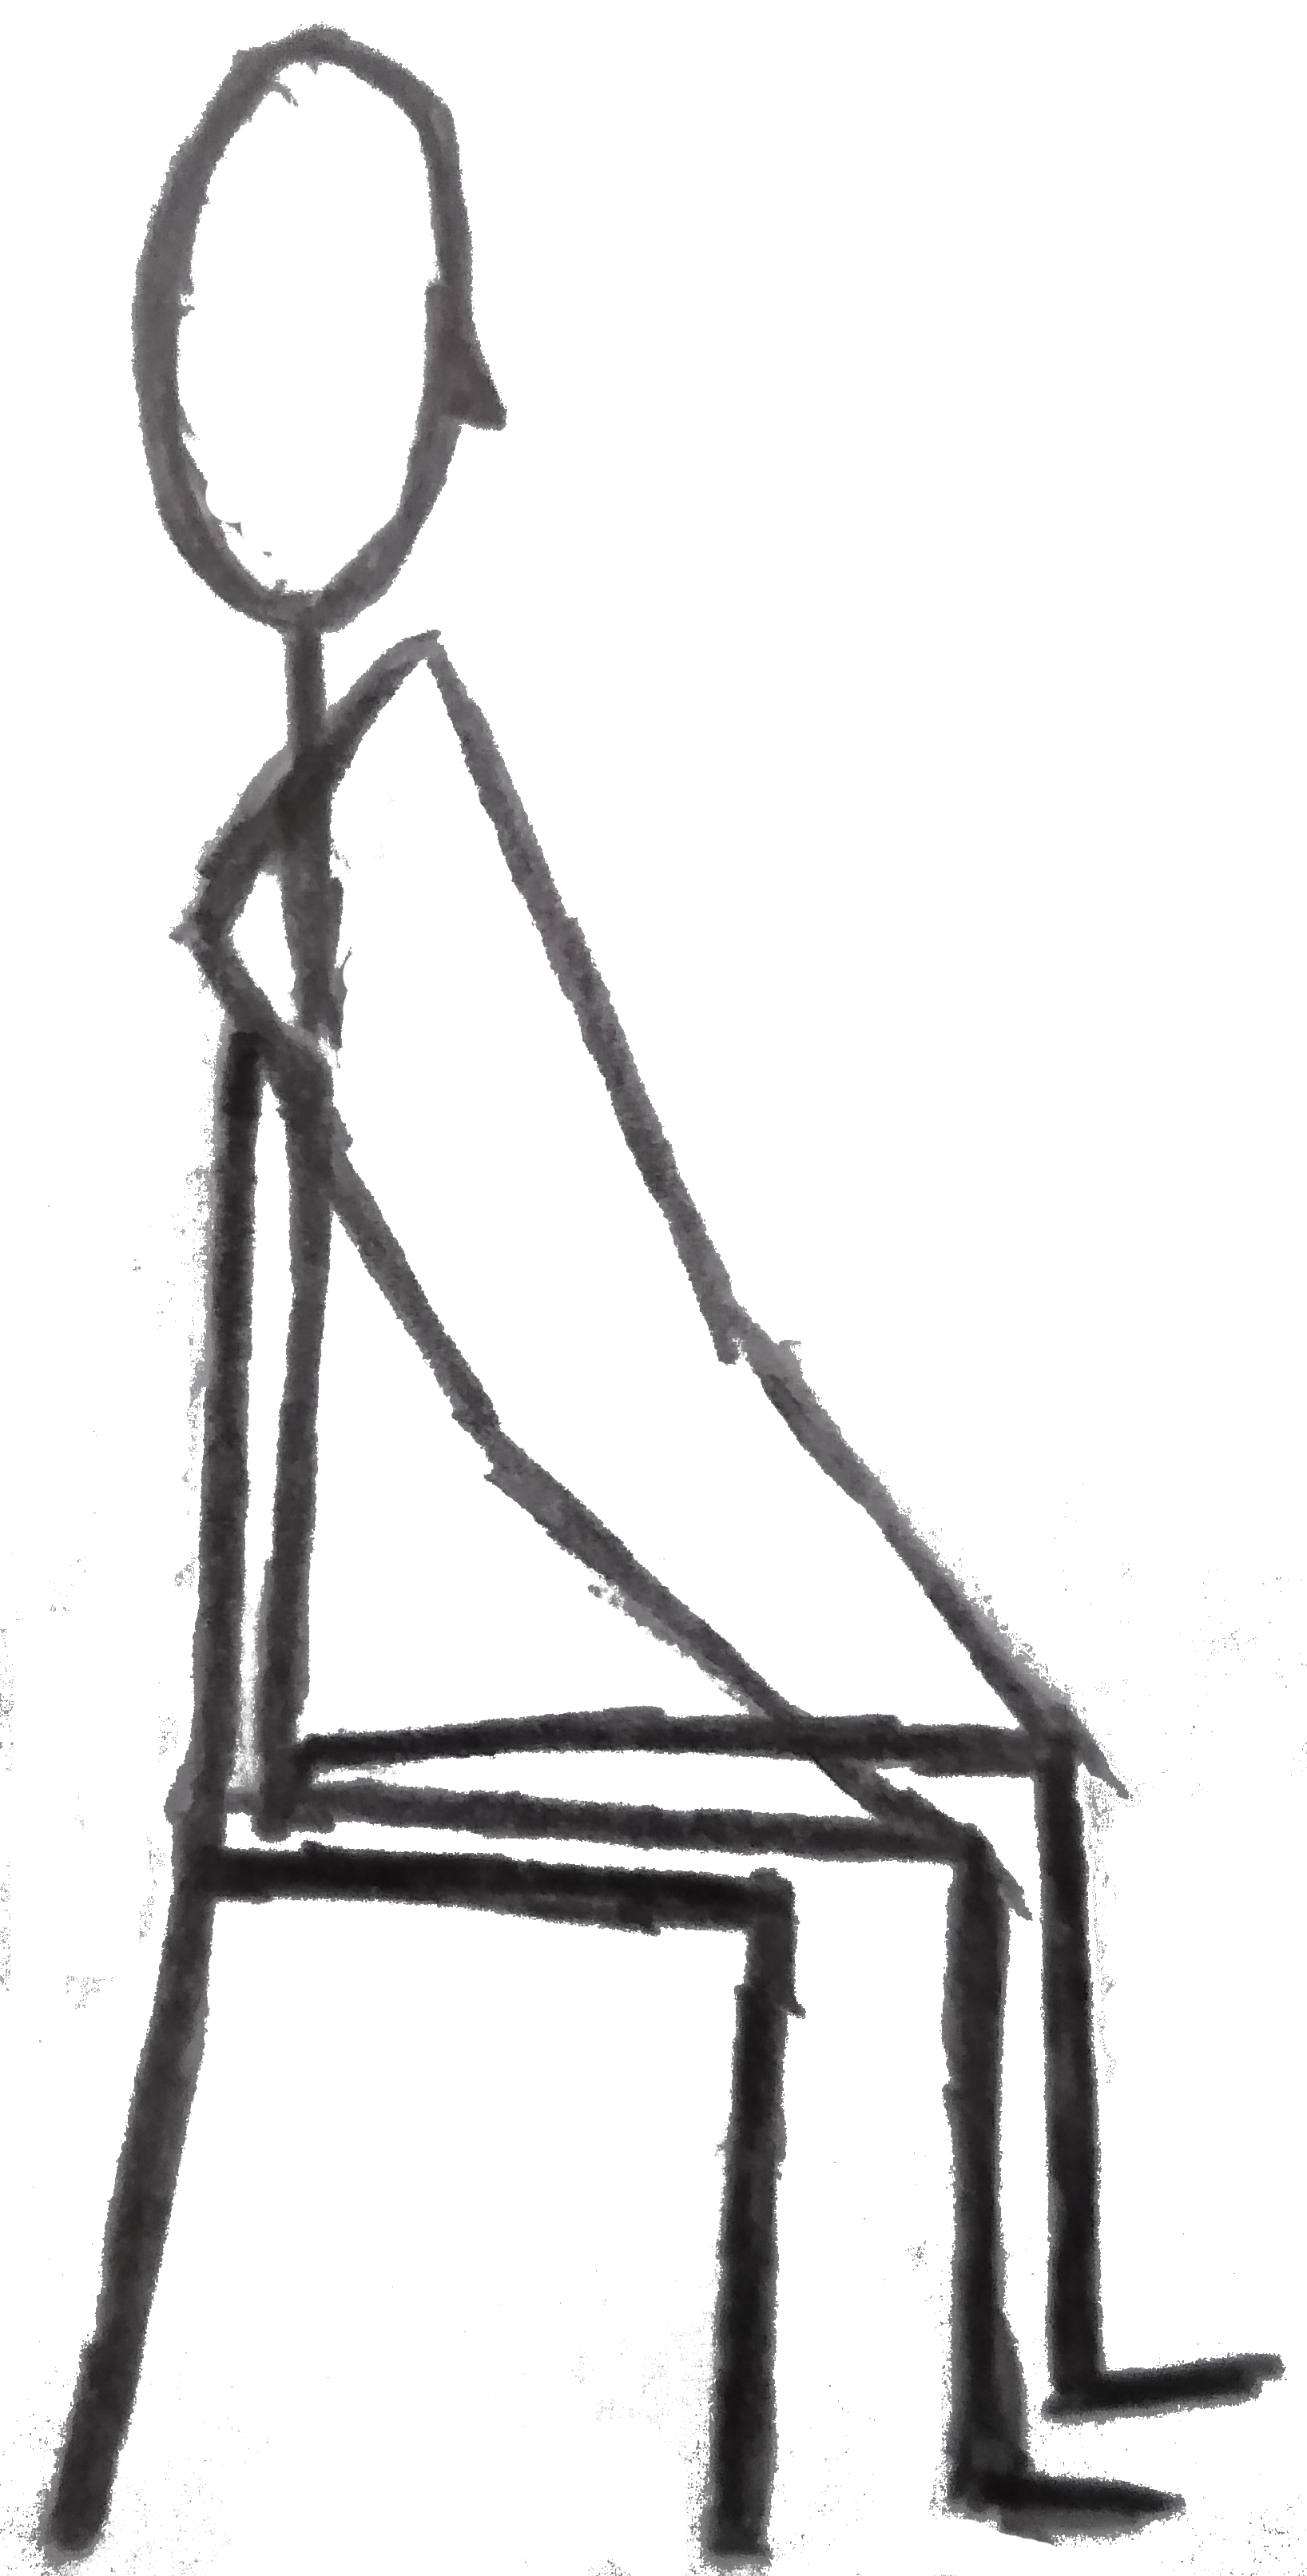
\includegraphics[width=1.7cm]{Sitting_chair_side}}\label{sf:sm_chair} & 
In the center of the formal practice is the sitting meditation\index{sitting meditation}.
In the {sitting meditation}, we {sit and breathe}.
Two activities we encounter everywhere in daily life. 
The sitting of the sitting meditation differs from the usual, daily sitting by the presence of our {inner mindful attitude}. 
In the sitting meditation it is important to sit in a {dignified posture},
with erect head, neck and back, without tensing up. 
You can use a chair with {straight back rest} or on a pillow on the {floor with your legs crossed}.
The position should radiate and {awake and dignified posture}. \\
 \raisebox{-0.65\totalheight}{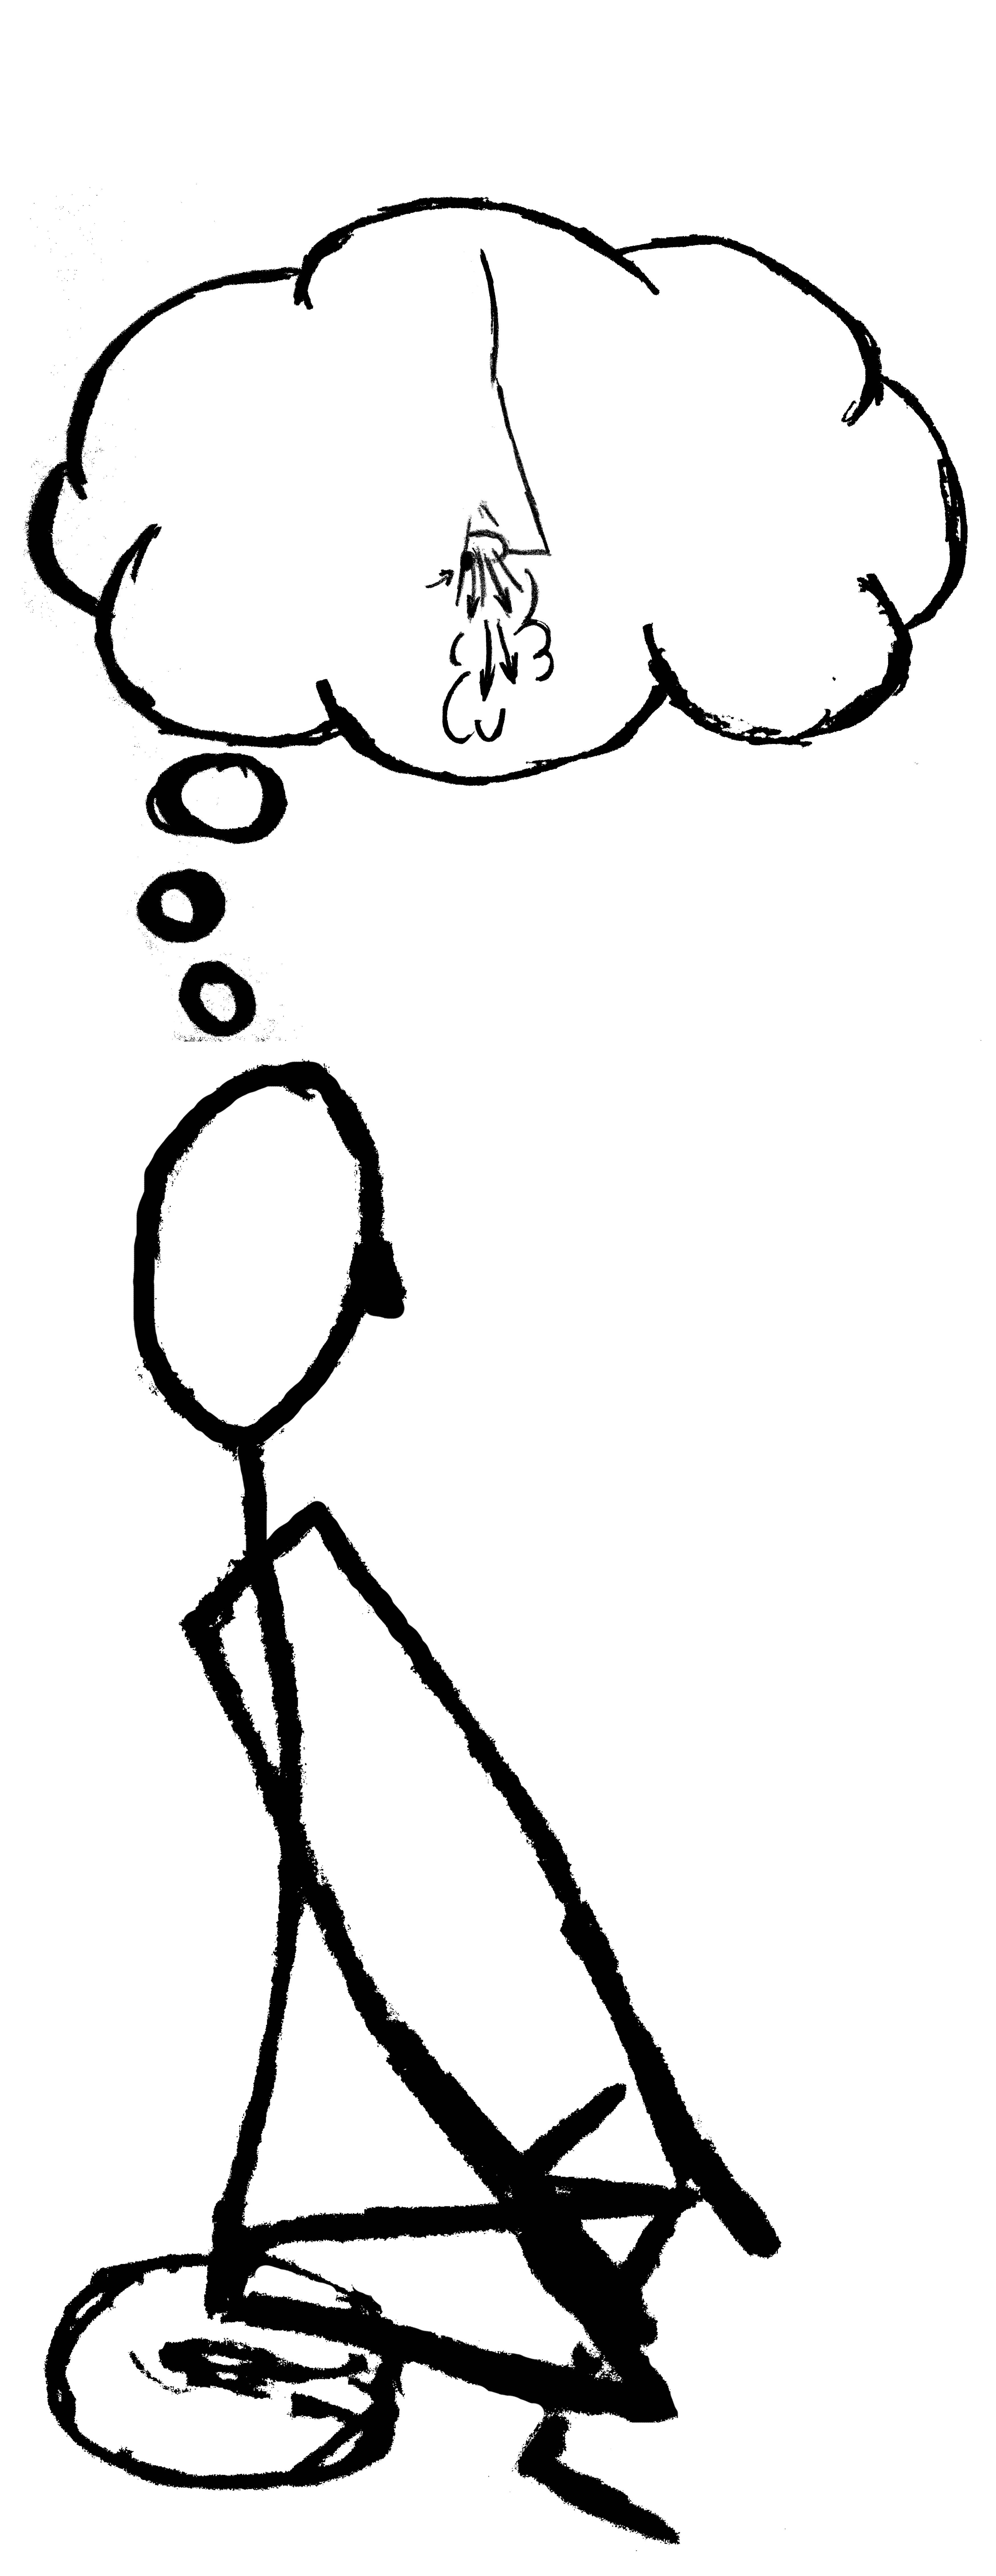
\includegraphics[width=1.9cm]{Thinking_man_breath}}\label{sf:sm_breath} & 
Normally you start by choosing an {object to focus the attention} - for instance your {breath}.\index{meditation!focus}
To be more precise, you focus on a single aspect of your breath,
like the sensation of the {air streaming in and out} at the back end of your nostrils
                                                                                   or the gentle {stretching and lowering of your abdominal wall} with each inhale and exhale.\\
 \raisebox{-0.65\totalheight}{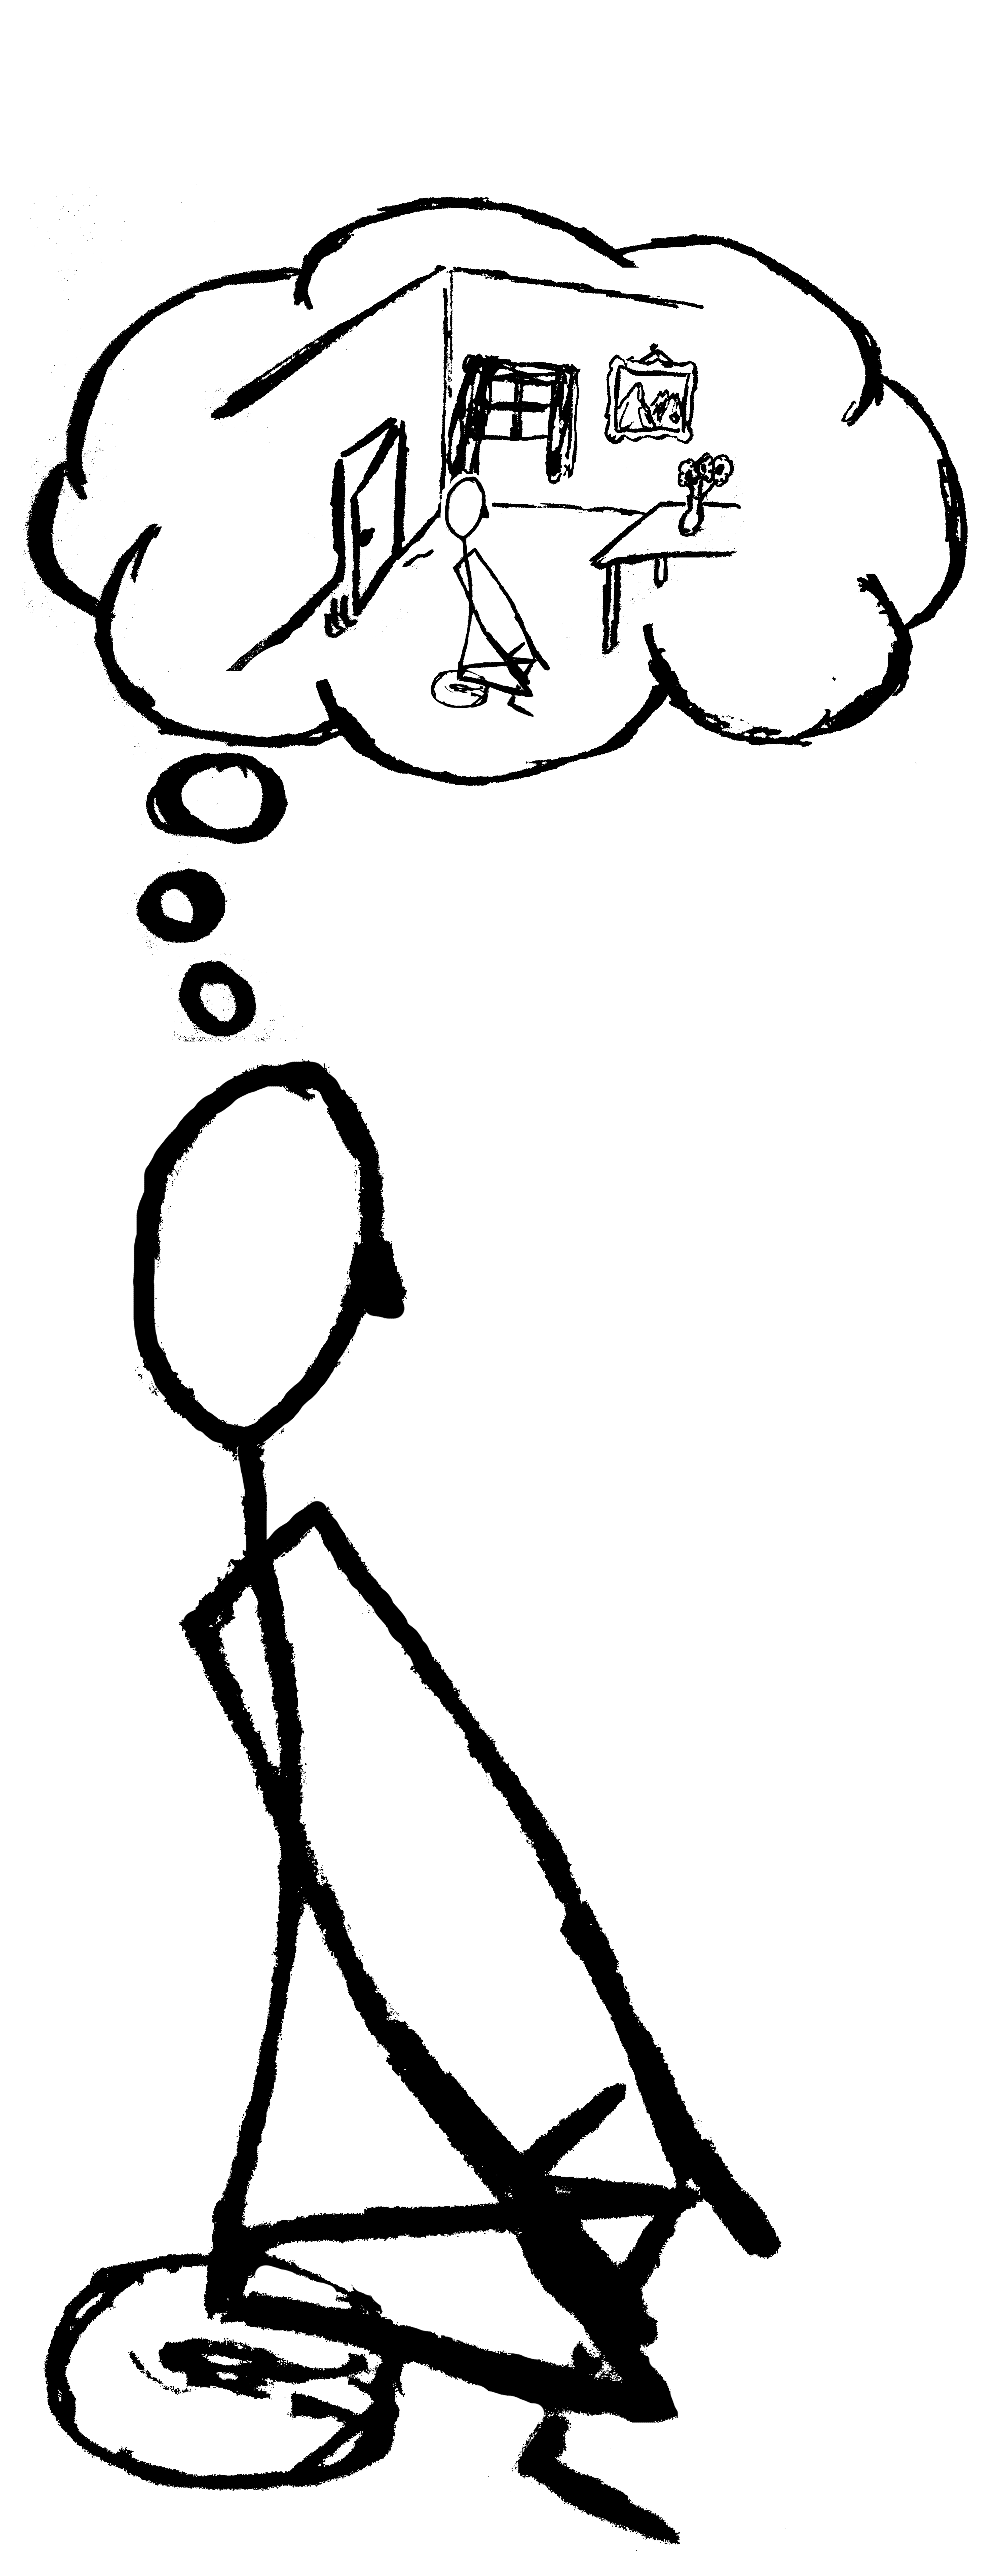
\includegraphics[width=1.9cm]{Thinking_man_thinkHouse}} & 
Once a certain degree of focus developed, the {attention can get widened} beyond the changing sensations of your breath.
                                                                                 
                                                                                Sounds, perceptions, thoughts or other objects will be perceived in a heedful manner as soon as they enter your awareness. We try as good as possible to maintain a {calm, non--reactive and steady awareness}, anchored by the breath.
\end{tabular}

\newpage
\subsubsection{What do you need for a sitting meditation?}

\begin{tabular}{p{1.8cm} p{9.7cm} }
 \raisebox{-1\totalheight}{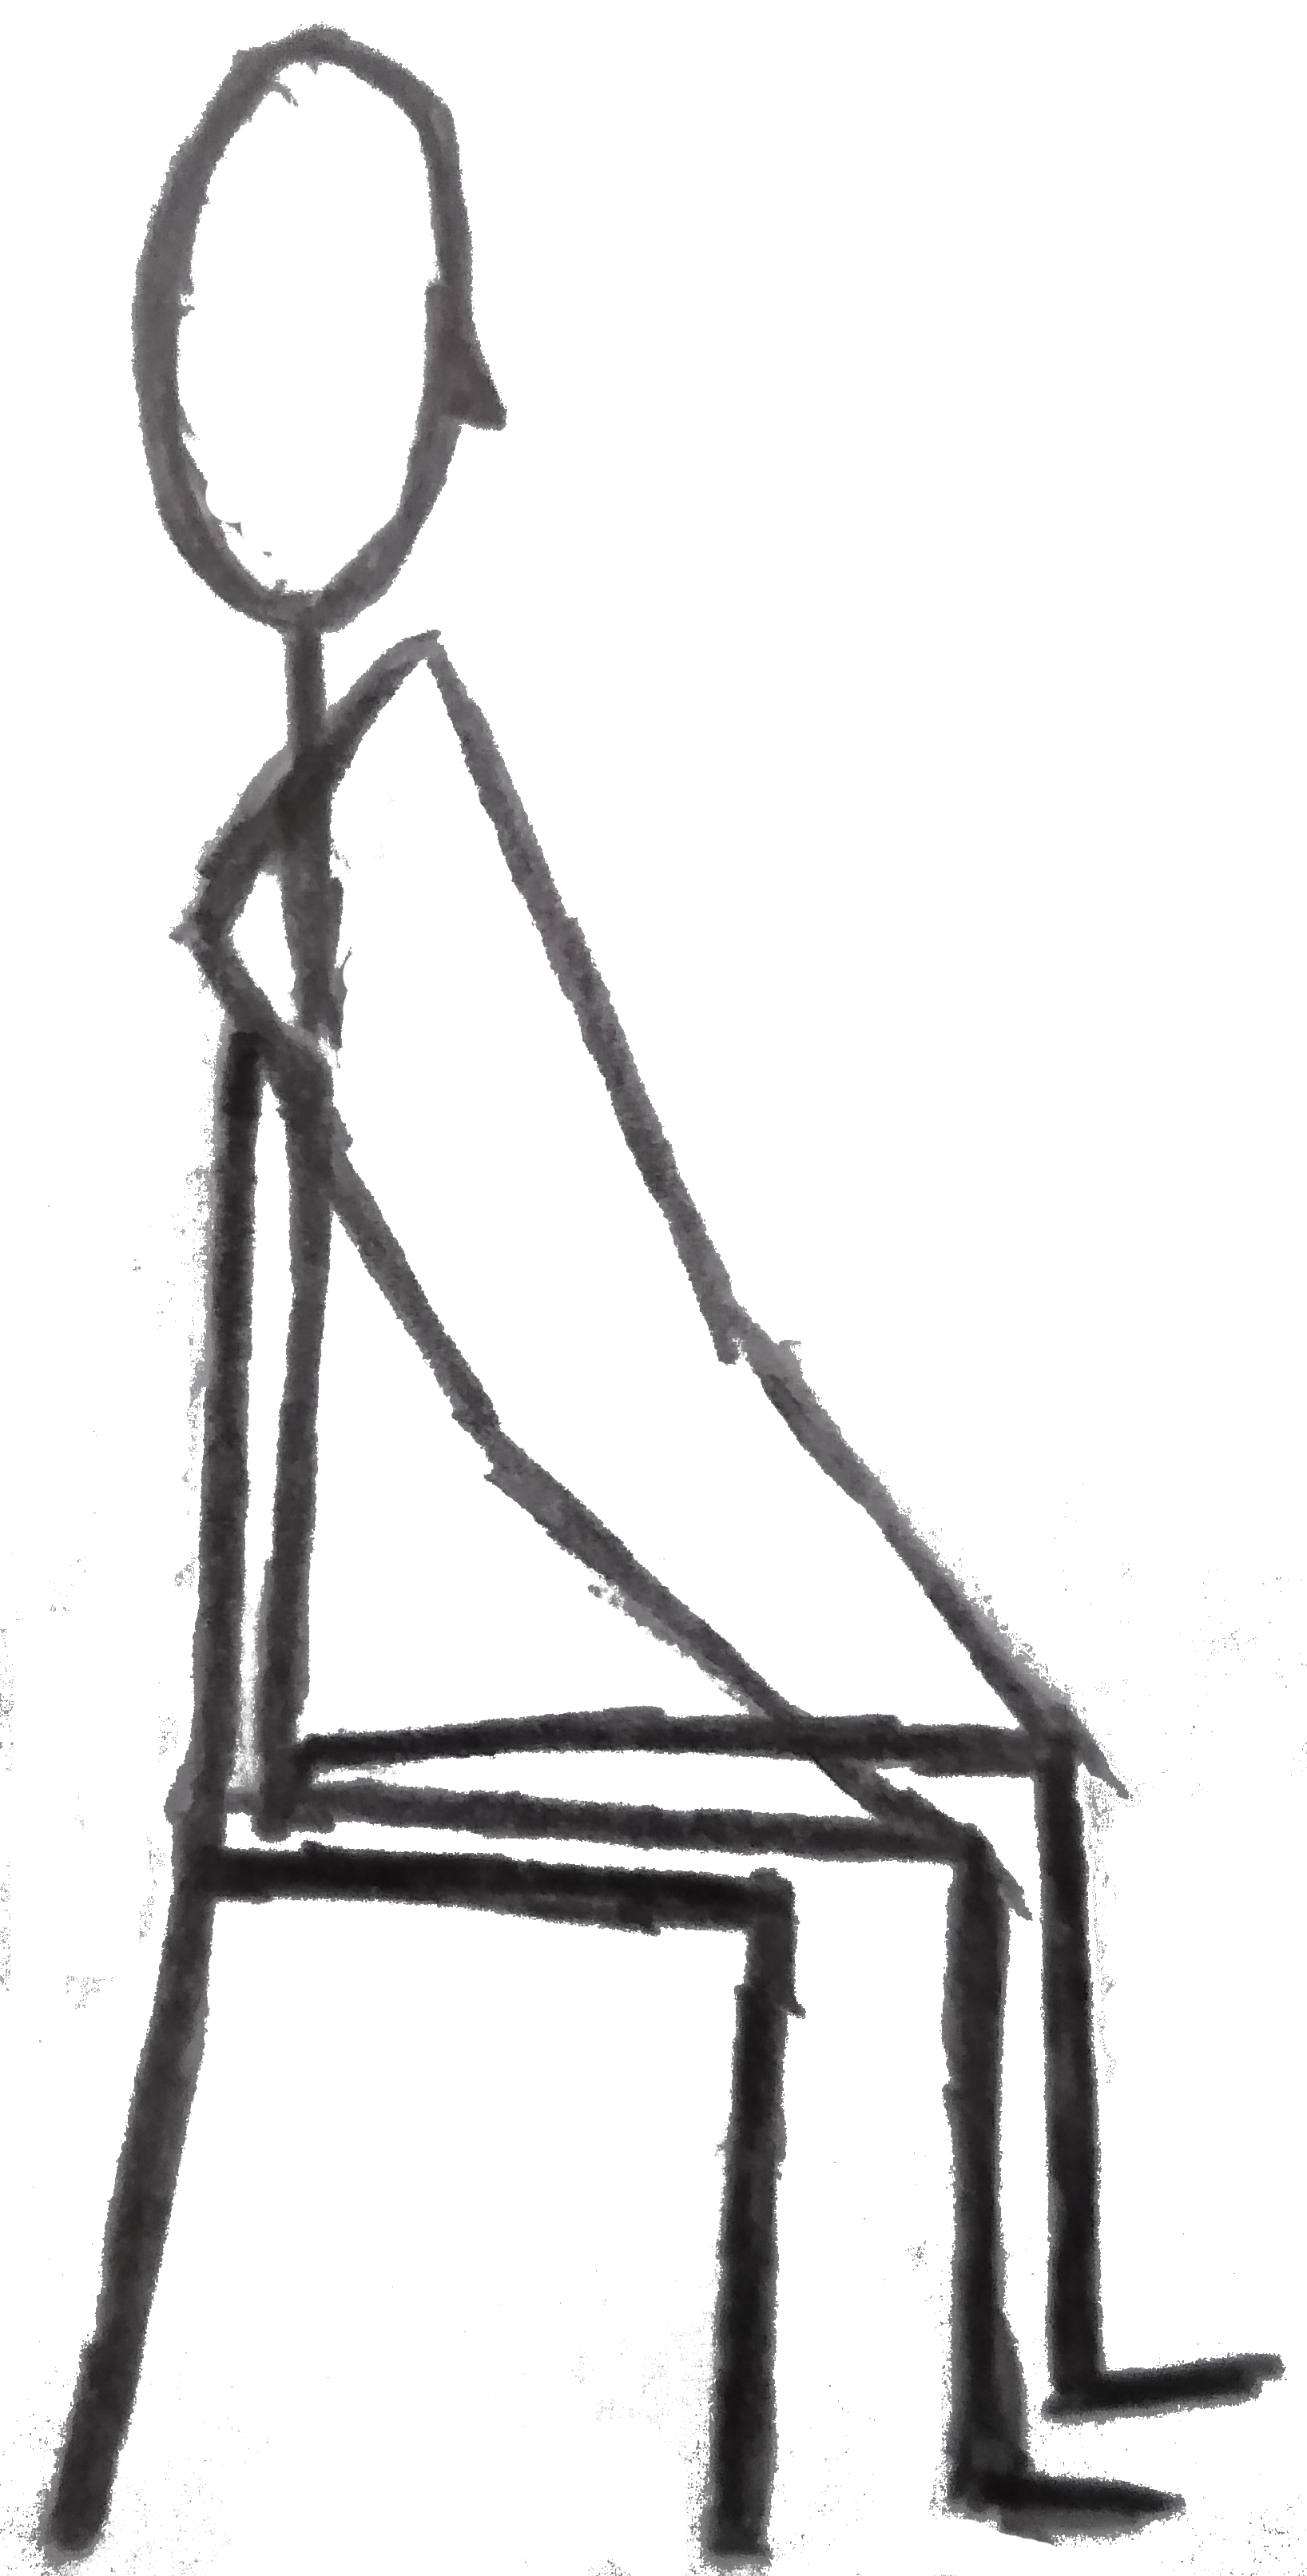
\includegraphics[width=1.8cm]{Sitting_chair_side}} & 

 A {fixed point of time}. 
 A place where you can relatively {undisturbed}. 
 An {upright posture} which allows you to sit for a prolonged period of time.\index{meditation!posture} 
 Find a seat on a chair with straight back rest or on the floor.
 If you sit on a chair, both {feet} should rest with the whole {soles on the floor}.
 Most of the time it’s indicated to not use the back rest, but to keep your {back free, straight and upright}.
 If this is too exhausting, then it’s preferable to lean against the backrest then to be constantly distracted by the unfamiliar strain. \\

  \raisebox{-1.2\totalheight}{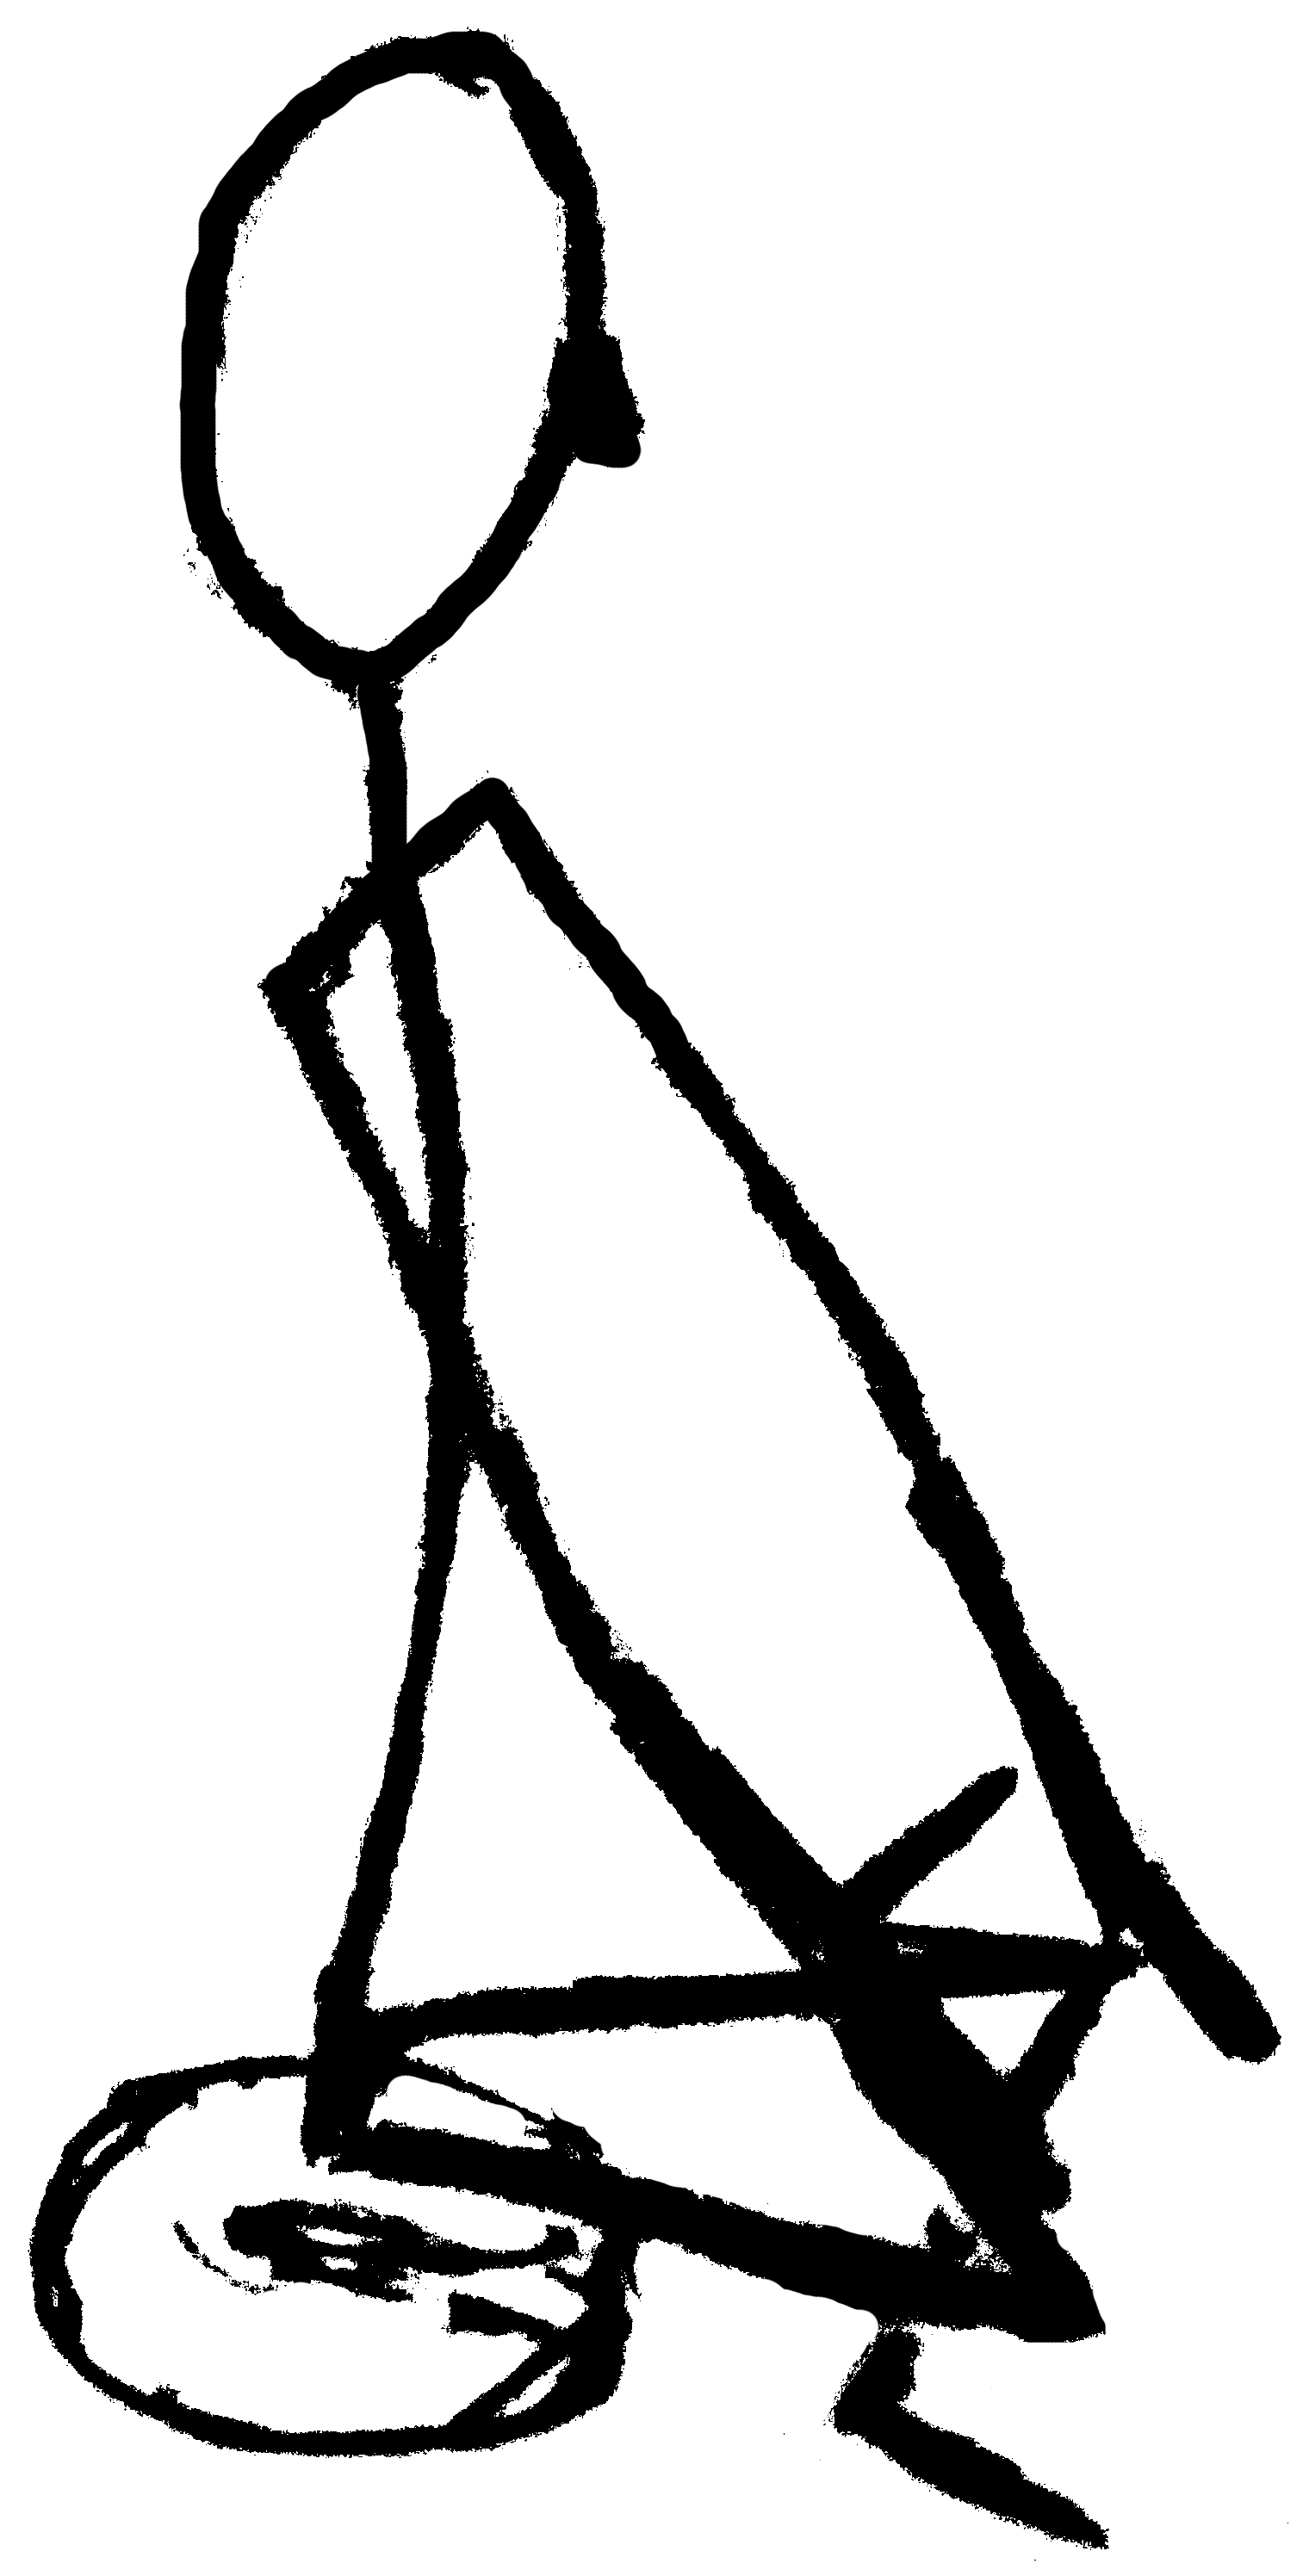
\includegraphics[width=1.6cm]{Sitting_floor_side}}&


                                                                                  When you sit on the floor, you can use a {pillow to lift the buttocks} off the floor (that helps to keep the back straight).
                                                                                  Take a {regular pillow} which you {fold} once or twice or then a special meditation pillow in wedge shape, a so called Zafu.
                                                                                  The position sitting on the floor can give you the calming feeling of being {stable and grounded}.



                                                                                  
                                                                                   Sitting on the floor isn't a condition for meditation, what really counts is the {sincerity of your efforts}, not the surface you're sitting on.
                                                                                                   It's recommendable that the {head, neck and back lie in a straight line} in order for the breath to flow effortlessly.
                                                                                                   This posture radiates a certain dignity and can progressively be an {expression of the inner attitude,
                                                                                                   your self esteem, self--acceptance and the focused attention} which you are about to cultivate. \end{tabular}

 \subsubsection{Follow the Breath}
 Did you settle down in a position? Put your attention on the {process of your breathing}.\index{meditation!breath}
 Feel consciously how the breath streams in and out.
 Let your breaths happen in a natural way and limit yourself to {observe it} and to {perceive all the related feelings}.
 Just take your sweet time and give your full attention to the inhale and the exhale.
 
\noindent
 \begin{tabular}{p{4.8cm} p{6.7cm} }
 \raisebox{-0.9\totalheight}{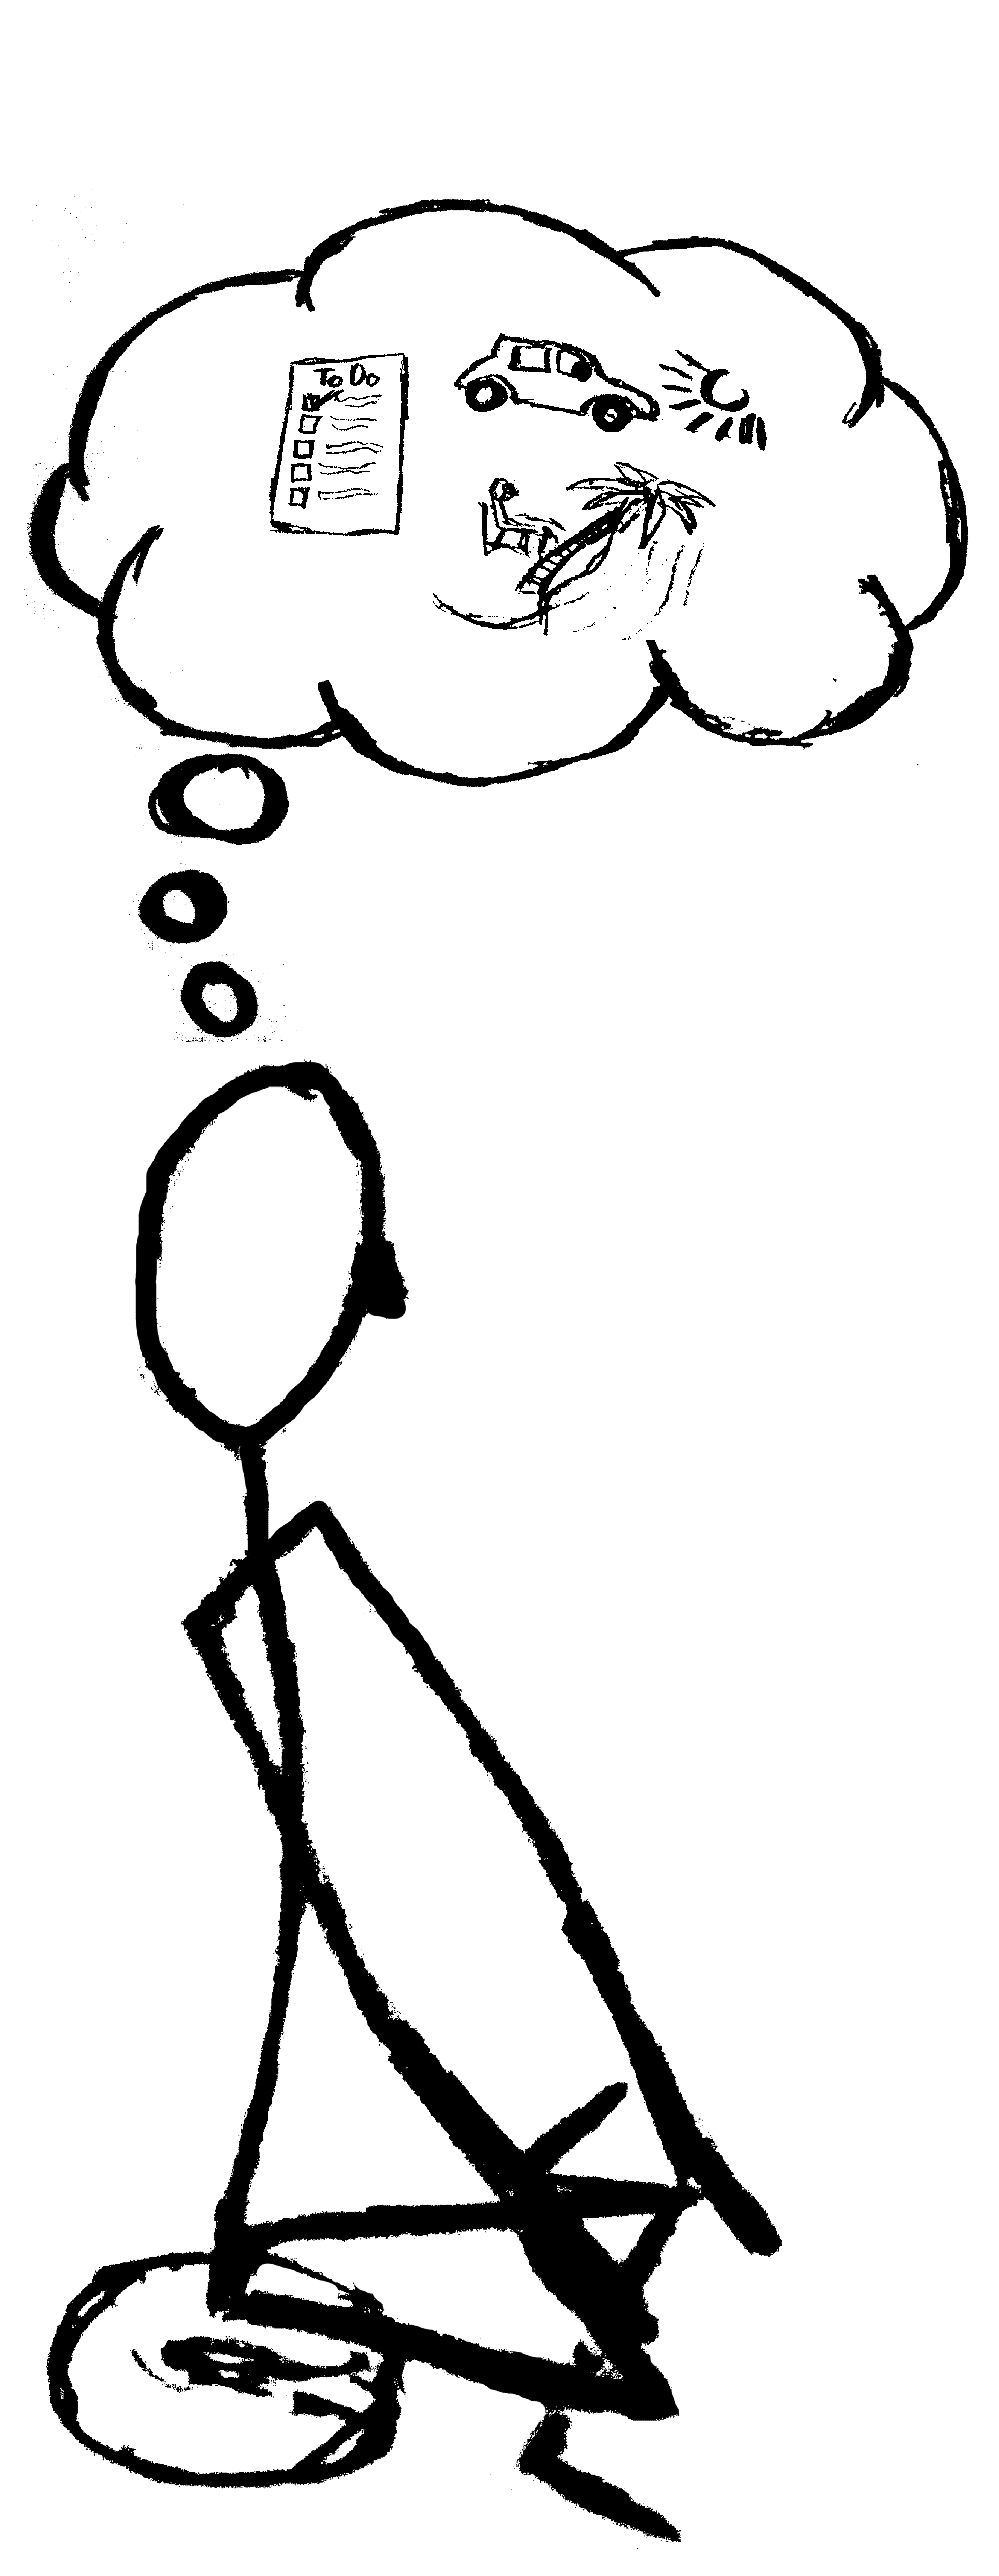
\includegraphics[width=1.8cm]{Thinking_mandistracted}} & 

Perhaps your body will urge you to to change the position, perhaps your {thoughts wander} to other topics.
That is totally {normal and unavoidable}.
In this case you can try to gently bring your attention back to your respiration, but in a determined way.
Don't let yourself {be distracted by your wandering thoughts} or by your restless body: {Stay patient} and don't get angry.
 \end{tabular}

 \subsubsection{The Basic Rules of the Sitting Meditation}

You will probably notice, that your {thoughts follow their own trajectories}: Even though you were seriously committed to  follow your breath, your {thoughts wandered} to other topics;
the conscious monitoring of your breath is forgotten.
Instead of getting upset, just try to continuously {lead your thoughts back to your breath}, without complaining about the digression.
Your thoughts are neither good nor bad.
In meditation it only counts if you’re {aware of your thoughts and how you deal with them}.
Don't try to suppress your thoughts, either: just {register their content and intensity} and let them {wander} by. 
Your thoughts are first and foremost {impulses, which you can follow} -- or not.
To recognize that can free us from the idea, that thoughts are uncontrollable realities.

The strongest distractions will come from your body.\index{meditation!distraction}
Again and again will you feel impulses, like stretching your leg or shifting your weight.
In meditation you should attempt to {resist these impulses}.
Take the {unease you're feeling as a given}.
Step by step you will still be able to meditate, regardless of the uncomfortable sensations.
At the last, you will learn this way how you can handle uncomfortable sensations  in a different manner.
Even though the sensations of your body can indeed be {uncomfortable}, you can still help them to unfold to {calm, serenity and focus}.
That's the only way to make the experience that {you can relax regardless of physical afflictions}.\index{unease!cope}
In case there's no other way and you really have to change posture: please do also this mindfully and focused.
\end{document}